% !TEX root = ../main.tex



\subsection{Inleiding}

\begin{frame}{Inleiding}
%\framesubtitle{}
\begin{figure}
\href{run:./media/Mythbusters-SoccerBallShotfromTruck.webm}{%
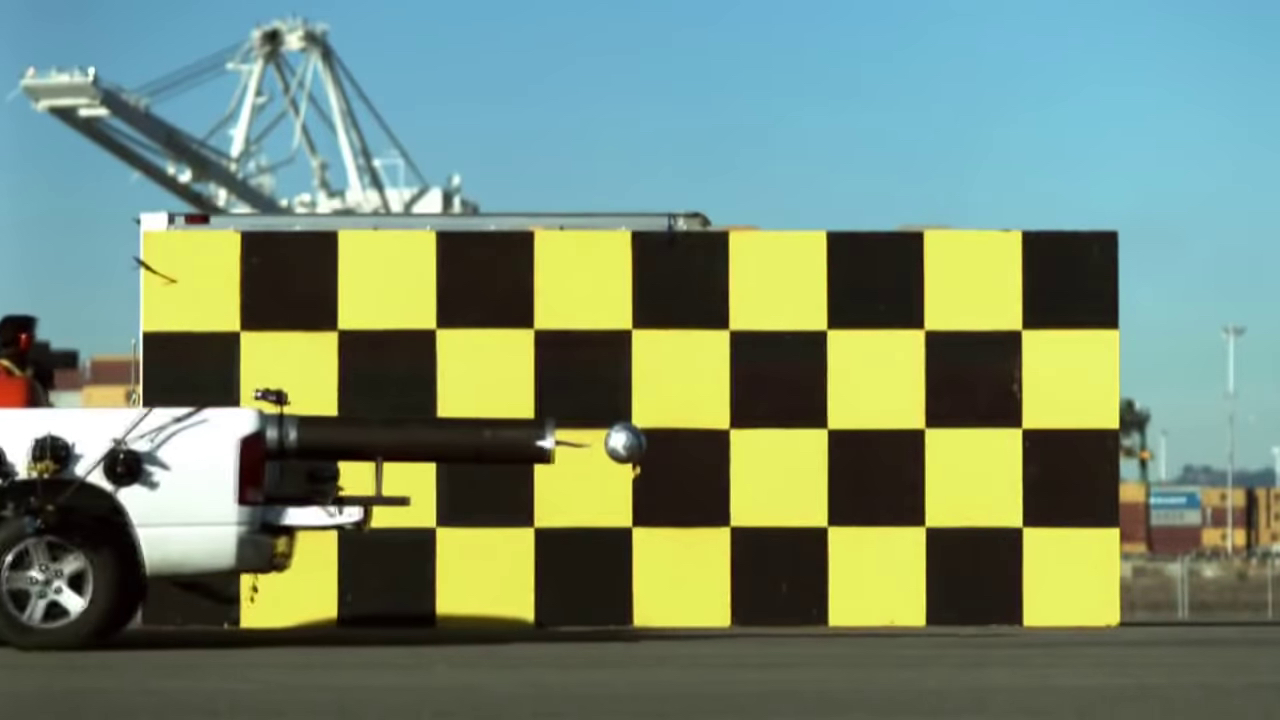
\includegraphics[height=\textheight-3\baselineskip]{vlcsnap-2022-09-25-20h21m15s386}
}
\end{figure}
\end{frame}
% Leerlingen zullen het niet moeilijk hebben met het idee dat de twee snelheden, die van de auto en die van de kogel, elkaar opheffen.
% Maar dan moet je het eens zijn met het idee dat de bal als het ware wordt losgelaten en zonder meer naar beneden valt.
% Neem je als referentie de auto, dan heeft de kogel wel een snelheid (hij wordt t.o.v. de auto met 60 mph? weggeschoten) die geen invloed kan hebben op de verticale valbeweging!


\subsection{Onafhankelijkheidsprincipe}

\subsection{Bewegingsvergelijking en baanvergelijking}

\begin{frame}{De horizontale worp}
\framesubtitle{}
\begin{figure}
\includegraphics<1>[height=\textheight-4\baselineskip]{horizontaleworp2}
\includegraphics<2>[height=\textheight-4\baselineskip]{horizontaleworp_valversnelling2}
\end{figure}
\end{frame}

\begin{frame}{Bewegingsvergelijking en baanvergelijking}
\framesubtitle{}
\end{frame}


\subsection{Oefeningen}

\usebackgroundtemplate{
\includegraphics[width=\paperwidth,height=\paperheight]{achtergrond22n_FV}}

\begin{frame}{Oefening 5 p. 90}
\begin{figure}
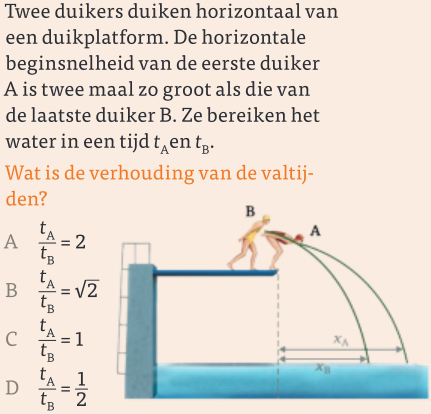
\includegraphics[height=\textheight-3\baselineskip]{5p90}
\end{figure}
\end{frame}

\begin{frame}{Oefening 10 p. 87}
\begin{figure}
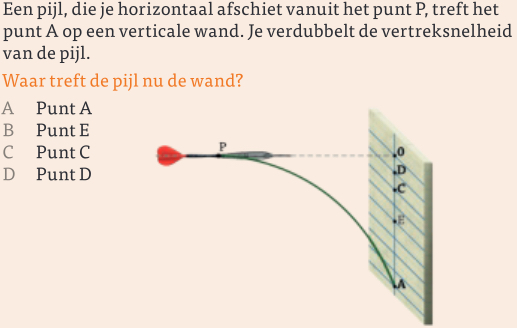
\includegraphics[height=\textheight-3\baselineskip]{10p87}
\end{figure}
\end{frame}

\begin{frame}{Oefening 14 p. 88}
\begin{figure}
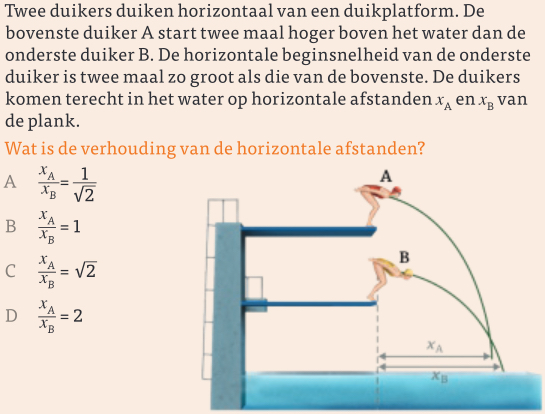
\includegraphics[height=\textheight-3\baselineskip]{14p88}
\end{figure}
\end{frame}

\begin{frame}{Oefening 5 p. 94}
\begin{figure}
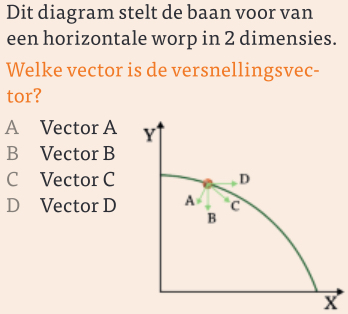
\includegraphics[height=\textheight-3\baselineskip]{5p94}
\end{figure}
\end{frame}

\usebackgroundtemplate{
\includegraphics[width=\paperwidth,height=\paperheight]{achtergrond22n}}